% CORTEX: Self-Evolving Cognitive Memory for Autonomous AI Agents
% LNCS Format — Springer
\documentclass[runningheads]{llncs}

\usepackage[T1]{fontenc}
\usepackage{graphicx}
\usepackage{amsmath,amssymb}
\usepackage{booktabs}
\usepackage{tikz}
\usetikzlibrary{positioning,arrows.meta,shapes.geometric,fit,calc,backgrounds,decorations.pathreplacing}
\usepackage[ruled,vlined,linesnumbered]{algorithm2e}
\usepackage{xcolor}
\usepackage{hyperref}
\usepackage{multirow}
\usepackage{tabularx}

% Compact lists
\usepackage{enumitem}
\setlist{nosep}

% Algorithm2e settings
\SetAlFnt{\small}
\SetAlCapFnt{\small}
\SetAlCapNameFnt{\small}

% Colors for diagrams
\definecolor{cortexblue}{HTML}{3B82F6}
\definecolor{cortexgreen}{HTML}{10B981}
\definecolor{cortexorange}{HTML}{F59E0B}
\definecolor{cortexpurple}{HTML}{8B5CF6}
\definecolor{cortexred}{HTML}{EF4444}
\definecolor{cortexgray}{HTML}{6B7280}
\definecolor{cortexteal}{HTML}{14B8A6}
\definecolor{cortexpink}{HTML}{EC4899}
\definecolor{cortexindigo}{HTML}{6366F1}

% Allow LaTeX more flexibility for line breaks
\emergencystretch=1em
\tolerance=1000

\begin{document}

\title{CORTEX: A Prompt-Aware Self-Evolving Cognitive Memory Architecture with Automatic Technique Selection for AI Agents}
\titlerunning{CORTEX: Self-Evolving Cognitive Memory}

\author{Anirach Mingkhwan\inst{1}}

\titlerunning{CORTEX: Prompt-Aware Self-Evolving Cognitive Memory}
\authorrunning{A. Mingkhwan}

\institute{King Mongkut's University of Technology North Bangkok, Bangkok, Thailand\\
\email{anirach.m@fitm.kmutnb.ac.th}}

\maketitle

%==============================================================
\begin{abstract}
While large language model (LLM)-based agents increasingly rely on persistent memory, existing systems treat memory as a passive store---retrieving content without adapting \textit{how} that content is presented to the LLM. We argue that \textbf{prompt-aware memory}---where the memory system itself selects and composes prompt engineering techniques based on task complexity---is essential for effective autonomous agents. We present \textbf{CORTEX} (Cognitive Orchestrated Retrieval with Temporal EXperience), which introduces a \textbf{PromptAssembler} module that automatically classifies queries into five complexity levels (simple, moderate, complex, knowledge gap, skill execution) and selects optimal combinations from ten prompt techniques including chain-of-thought, ReAct, few-shot from procedural memory, and self-critique---with outcome recording that enables the system to learn which assemblies produce better results over time. The PromptAssembler operates atop a nine-layer cognitive memory architecture featuring four biologically-inspired memory types, a hippocampal hybrid search index, Ebbinghaus forgetting curves, sleep/dream consolidation, genetic algorithm-based retrieval evolution, active gap filling, multi-backend semantic embeddings (ONNX/sentence-transformers with hash fallback), and bidirectional Obsidian vault synchronization. CORTEX operates offline with zero mandatory external dependencies. Evaluation across 179 unit tests demonstrates correctness with sub-millisecond operations, convergent evolution within 10 generations, and measurably improved recall with semantic embeddings over hash-based baselines.

\keywords{Prompt engineering \and Cognitive memory architecture \and Autonomous agents \and Self-evolving AI \and Prompt assembly \and Memory consolidation}
\end{abstract}

%==============================================================
\section{Introduction}\label{sec:intro}

The emergence of LLM-based autonomous agents~\cite{weng2023agent,sumers2023cognitive} has created an urgent need for persistent, structured memory systems. While recent work has produced capable memory stores---Mem0~\cite{mem0_2024} for fact extraction, MemGPT/Letta~\cite{packer2023memgpt} for virtual context management, Zep~\cite{zep2024} for temporal memory---these systems share a critical blind spot: they retrieve content but have no awareness of \textit{how} that content should be presented to the LLM. A simple factual lookup and a complex multi-step analysis both receive the same flat context injection.

Human cognition does not work this way. When recalling information for a simple question (``What year was that?''), we retrieve directly. For complex reasoning (``Why did this policy fail?''), we engage step-by-step analysis, draw on analogies, and self-critique our conclusions. The \textit{mode of retrieval and presentation} adapts to task demands~\cite{tulving1972episodic,squire2004memory,baddeley2000working}.

Current agent memory systems suffer from four key limitations: (1)~they lack multi-type memory organization inspired by cognitive science, (2)~they have no self-evolution mechanism for retrieval strategies, (3)~they do not actively detect and fill knowledge gaps, and (4)~\textbf{they are prompt-unaware}---incapable of adapting their output format, reasoning structure, or technique composition to match task complexity. Furthermore, no existing system provides bidirectional synchronization with personal knowledge management tools.

\textbf{Contributions.} We introduce CORTEX, a prompt-aware cognitive memory architecture that addresses these gaps. Our primary contribution is:

\begin{enumerate}[leftmargin=*]
    \item \textbf{Prompt-aware cognitive assembly (PromptAssembler)}---the first memory system that automatically classifies task complexity into five levels and selects optimal combinations from ten prompt engineering techniques (chain-of-thought, ReAct, few-shot from procedural memory, self-critique, role prompting, etc.), with outcome recording that enables the system to learn which assemblies work best over time.
\end{enumerate}

\noindent This PromptAssembler operates atop a comprehensive cognitive memory foundation with six additional contributions:

\begin{enumerate}[leftmargin=*]\setcounter{enumi}{1}
    \item \textbf{Unified multi-type memory} with four biologically-inspired stores (working, episodic, semantic, procedural) connected through a hippocampal hybrid search index combining vector similarity, BM25, temporal, graph, and importance signals.
    \item \textbf{Cognitive lifecycle management} via an Ebbinghaus forgetting curve ($R = e^{-t/S}$) and a sleep/dream consolidation cycle that promotes memories across types.
    \item \textbf{Self-evolution} through a genetic algorithm that evolves retrieval strategy parameters using tournament selection with elitism, producing measurable fitness convergence.
    \item \textbf{Active knowledge gap filling} with a four-class taxonomy (inferrable, searchable, askable, consolidatable) and five auto-fill strategies.
    \item \textbf{Bidirectional Obsidian vault synchronization} supporting PARA method detection, wikilink graph mapping, dead link gap detection, and auto-generated Maps of Content.
    \item \textbf{Multi-backend semantic embeddings} with automatic detection (ONNX Runtime, sentence-transformers, or hash-based TF-IDF fallback), enabling real semantic understanding without mandatory external dependencies.
\end{enumerate}

%==============================================================
\section{Related Work}\label{sec:related}

\subsection{Memory Systems for AI Agents}

\textbf{Mem0}~\cite{mem0_2024} provides a memory layer that automatically extracts and stores facts from conversations, supporting graph-based relationships. However, it lacks multi-type memory organization and self-evolution.
\textbf{MemGPT/Letta}~\cite{packer2023memgpt} treats LLMs as operating systems with virtual context management, implementing main and archival memory tiers. It does not support procedural memory or forgetting curves.
\textbf{Zep}~\cite{zep2024} offers long-term memory with temporal awareness and entity extraction but lacks consolidation cycles and self-improvement.
\textbf{Hindsight}~\cite{hindsight2024} implements self-improving memory through reflection but does not incorporate genetic evolution or gap filling.
\textbf{Cognee}~\cite{cognee2024} provides graph-based RAG with deterministic outputs but focuses on retrieval rather than cognitive memory management.

Recent surveys~\cite{zhang2024survey,hatalis2023memory} identify memory management as a critical open problem, with no existing system combining all four cognitive memory types with self-evolution.

\subsection{Cognitive Architectures}

Classical cognitive architectures provide theoretical foundations. \textbf{ACT-R}~\cite{anderson2004act} models human cognition with declarative and procedural modules, inspiring our dual long-term memory design. \textbf{SOAR}~\cite{laird2012soar} implements production rules and chunking, analogous to our procedural memory with reliability tracking. \textbf{Global Workspace Theory}~\cite{baars2005gwt} posits a shared workspace for competing cognitive processes, reflected in our hippocampal index that arbitrates across memory types. Park et al.~\cite{park2023generative} demonstrated generative agents with reflection and planning using memory streams, while Sumers et al.~\cite{sumers2023cognitive} formalized cognitive architectures for language agents.

\subsection{Knowledge Management Methods}

The \textbf{Second Brain} methodology~\cite{forte2022second} and the \textbf{PARA} method (Projects, Areas, Resources, Archive) provide organizational frameworks that CORTEX detects and maps to memory types during Obsidian vault ingestion. The \textbf{Zettelkasten} method~\cite{ahrens2017zettelkasten} emphasizes atomic, interlinked notes---a structure our wikilink graph parser naturally captures.

\subsection{Agent Frameworks}

Modern agent frameworks including AutoGen~\cite{wu2023autogen}, CrewAI~\cite{crewai2024}, LangGraph~\cite{langgraph2024}, and OpenClaw~\cite{openclaw2025} provide orchestration for multi-agent systems but delegate memory management to external stores. CORTEX is designed as an embeddable memory engine for any such framework.

\subsection{Self-Improving AI Systems}

Voyager~\cite{wang2023voyager} maintains a skill library that grows through exploration, similar to our procedural memory. Reflexion~\cite{shinn2023reflexion} uses verbal reinforcement learning from mistakes, paralleling our self-improvement engine. MemoryBank~\cite{hu2024memorybank} applies forgetting curves to LLM memory but lacks multi-type organization and evolution. Neural Turing Machines~\cite{graves2014neural} and End-to-End Memory Networks~\cite{sukhbaatar2015end} provide differentiable memory access but operate at the neural network level rather than the agent architecture level.

%==============================================================
\section{CORTEX Architecture}\label{sec:arch}

CORTEX comprises nine interconnected layers orchestrated by a central \texttt{CortexEngine} class. Figure~\ref{fig:architecture} presents the overall architecture.

% ── Architecture Diagram ──────────────────────────────────
\begin{figure}[t]
\centering
\resizebox{\textwidth}{!}{%
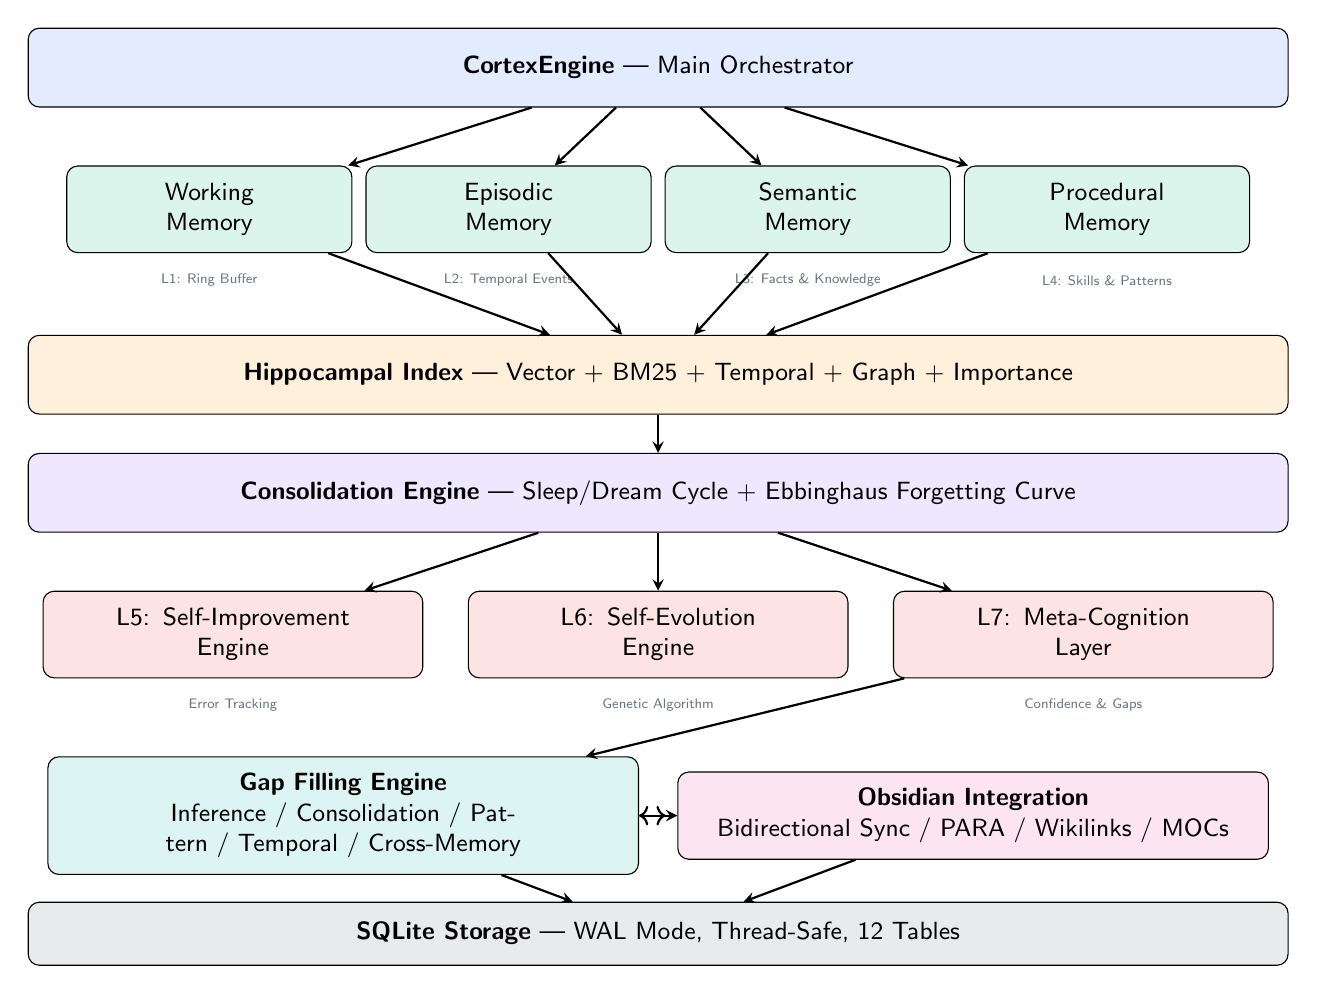
\begin{tikzpicture}[
    layer/.style={draw, rounded corners=4pt, minimum height=1.1cm, align=center, font=\small\sffamily, inner sep=6pt},
    arrow/.style={-stealth, thick},
    darrow/.style={<->stealth, thick},
    label/.style={font=\tiny\sffamily, text=cortexgray},
]

% Row 1: Orchestrator
\node[layer, fill=cortexblue!15, minimum width=16cm, minimum height=1.0cm] (engine) at (0,0) {\textbf{CortexEngine} --- Main Orchestrator};

% Row 2: Four memory types
\node[layer, fill=cortexgreen!15, minimum width=3.6cm, text width=3.2cm] (working) at (-5.7,-1.8) {Working\\Memory};
\node[layer, fill=cortexgreen!15, minimum width=3.6cm, text width=3.2cm] (episodic) at (-1.9,-1.8) {Episodic\\Memory};
\node[layer, fill=cortexgreen!15, minimum width=3.6cm, text width=3.2cm] (semantic) at (1.9,-1.8) {Semantic\\Memory};
\node[layer, fill=cortexgreen!15, minimum width=3.6cm, text width=3.2cm] (procedural) at (5.7,-1.8) {Procedural\\Memory};

\node[label] at (-5.7,-2.7) {L1: Ring Buffer};
\node[label] at (-1.9,-2.7) {L2: Temporal Events};
\node[label] at (1.9,-2.7) {L3: Facts \& Knowledge};
\node[label] at (5.7,-2.7) {L4: Skills \& Patterns};

% Row 3: Hippocampal Index
\node[layer, fill=cortexorange!15, minimum width=16cm, minimum height=1.0cm] (hippo) at (0,-3.9) {\textbf{Hippocampal Index} --- Vector + BM25 + Temporal + Graph + Importance};

% Row 4: Consolidation + Forgetting
\node[layer, fill=cortexpurple!15, minimum width=16cm, minimum height=1.0cm] (consol) at (0,-5.4) {\textbf{Consolidation Engine} --- Sleep/Dream Cycle + Ebbinghaus Forgetting Curve};

% Row 5: Three cognitive layers
\node[layer, fill=cortexred!15, minimum width=4.8cm, text width=4.4cm] (improve) at (-5.4,-7.2) {L5: Self-Improvement\\Engine};
\node[layer, fill=cortexred!15, minimum width=4.8cm, text width=4.4cm] (evolution) at (0,-7.2) {L6: Self-Evolution\\Engine};
\node[layer, fill=cortexred!15, minimum width=4.8cm, text width=4.4cm] (metacog) at (5.4,-7.2) {L7: Meta-Cognition\\Layer};

\node[label] at (-5.4,-8.1) {Error Tracking};
\node[label] at (0,-8.1) {Genetic Algorithm};
\node[label] at (5.4,-8.1) {Confidence \& Gaps};

% Row 6: Gap Filling + Obsidian
\node[layer, fill=cortexteal!15, minimum width=7.5cm, text width=7.0cm] (gapfill) at (-4.0,-9.5) {\textbf{Gap Filling Engine}\\Inference / Consolidation / Pattern / Temporal / Cross-Memory};
\node[layer, fill=cortexpink!15, minimum width=7.5cm, text width=7.0cm] (obsidian) at (4.0,-9.5) {\textbf{Obsidian Integration}\\Bidirectional Sync / PARA / Wikilinks / MOCs};

% Row 7: Storage
\node[layer, fill=cortexgray!15, minimum width=16cm, minimum height=0.8cm] (storage) at (0,-11.0) {\textbf{SQLite Storage} --- WAL Mode, Thread-Safe, 12 Tables};

% Arrows
\foreach \mem in {working, episodic, semantic, procedural} {
    \draw[arrow] (engine) -- (\mem);
    \draw[arrow] (\mem) -- (hippo);
}
\draw[arrow] (hippo) -- (consol);
\draw[arrow] (consol) -- (improve);
\draw[arrow] (consol) -- (evolution);
\draw[arrow] (consol) -- (metacog);
\draw[arrow] (metacog) -- (gapfill);
\draw[darrow] (gapfill) -- (obsidian);
\draw[arrow] (gapfill) -- (storage);
\draw[arrow] (obsidian) -- (storage);

\end{tikzpicture}
}
\caption{CORTEX nine-layer cognitive memory architecture. Layers L1--L4 provide multi-type storage; the hippocampal index unifies retrieval; the consolidation engine manages memory lifecycle; layers L5--L7 provide self-awareness; gap filling and Obsidian integration connect to external knowledge.}
\label{fig:architecture}
\end{figure}

\subsection{Layer 1: Working Memory}\label{sec:working}

Working memory implements a fixed-capacity ring buffer (class \texttt{WorkingMemory}, default capacity $C=20$) that maintains the agent's immediate context. When the buffer is full, the oldest item is evicted via FIFO. Each \texttt{WorkingItem} stores content, metadata, a creation timestamp, and a slot number. The \texttt{push}, \texttt{get\_recent(n)}, \texttt{search(query)}, and \texttt{clear()} operations execute in $O(1)$, $O(n)$, $O(C)$, and $O(C)$ time respectively. During consolidation, all working memory items are flushed to episodic memory.

\subsection{Layer 2: Episodic Memory}\label{sec:episodic}

Episodic memory (class \texttt{EpisodicMemory}) stores timestamped events as \texttt{Episode} dataclasses with fields: \texttt{id}, \texttt{content}, \texttt{embedding} (256-dimensional hash vector), \texttt{importance} $\in [0,1]$, \texttt{access\_count}, \texttt{last\_accessed}, \texttt{tags}, and \texttt{source}. Retrieval combines cosine similarity with retention scoring:
\begin{equation}\label{eq:episodic-score}
    \text{score}(e, q) = \text{sim}(\mathbf{v}_e, \mathbf{v}_q) \cdot R(e) \cdot (0.5 + \text{importance}(e))
\end{equation}
where $R(e)$ is the Ebbinghaus retention (Section~\ref{sec:forgetting}). Episodes below a minimum retention threshold are excluded from retrieval. Access timestamps are updated on every retrieval (spaced repetition effect).

\subsection{Layer 3: Semantic Memory}\label{sec:semantic}

Semantic memory (class \texttt{SemanticMemory}) stores \texttt{Fact} objects with additional fields: \texttt{category}, \texttt{confidence} $\in [0,1]$, and optional filtering by category and minimum confidence. The scoring function is:
\begin{equation}\label{eq:semantic-score}
    \text{score}(f, q) = \text{sim}(\mathbf{v}_f, \mathbf{v}_q) \cdot \text{confidence}(f) \cdot (0.5 + \text{importance}(f))
\end{equation}
Categories enable topic-organized retrieval, while the confidence field allows uncertain or inferred knowledge to coexist with verified facts.

\subsection{Layer 4: Procedural Memory}\label{sec:procedural}

Procedural memory (class \texttt{ProceduralMemory}) stores \texttt{Skill} objects with \texttt{pattern}, \texttt{trigger}, \texttt{success\_count}, and \texttt{failure\_count} fields. Reliability uses Laplace-smoothed Bayesian estimation:
\begin{equation}\label{eq:reliability}
    \text{reliability}(s) = \frac{s_{\text{success}} + 1}{s_{\text{success}} + s_{\text{failure}} + 2}
\end{equation}
Retrieval scoring weights similarity by reliability:
\begin{equation}\label{eq:proc-score}
    \text{score}(s, q) = \text{sim}(\mathbf{v}_s, \mathbf{v}_q) \cdot \text{reliability}(s) \cdot (0.5 + \text{importance}(s))
\end{equation}
The \texttt{record\_outcome(skill\_id, success)} method tracks real-world performance. The \texttt{get\_by\_trigger(query)} method enables automatic skill selection via trigger matching.

\subsection{Hippocampal Index: Hybrid Search}\label{sec:hippo}

The \texttt{HippocampalIndex} class unifies retrieval across all three persistent memory types by combining five signals into a single relevance score (Figure~\ref{fig:hippocampus}):

\begin{equation}\label{eq:hybrid}
    S(m, q) = \sum_{k \in \mathcal{K}} w_k \cdot s_k(m, q)
\end{equation}

where $\mathcal{K} = \{\text{similarity}, \text{bm25}, \text{temporal}, \text{graph}, \text{importance}\}$ and the weights $w_k$ are controlled by the evolved retrieval strategy (Section~\ref{sec:evolution}).

\begin{figure}[t]
\centering
\resizebox{\textwidth}{!}{%
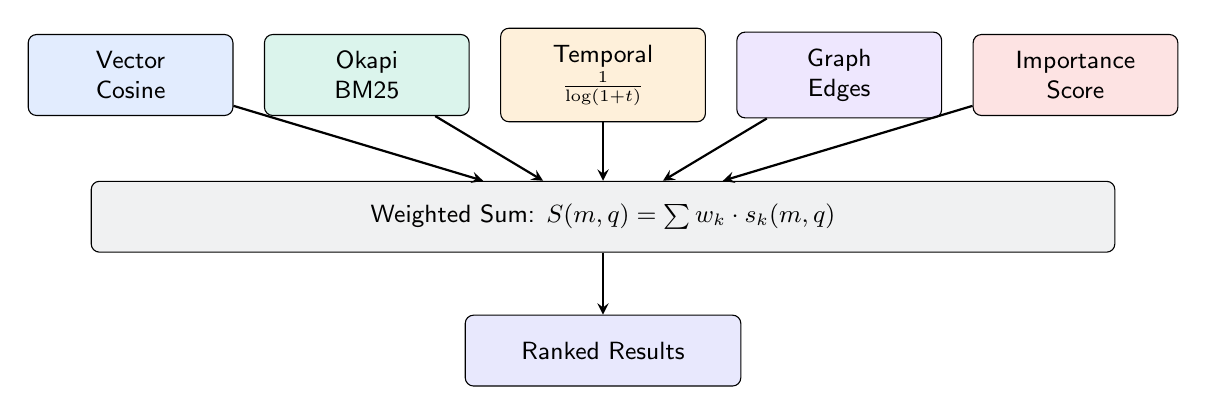
\begin{tikzpicture}[
    signal/.style={draw, rounded corners=3pt, fill=#1!15, minimum width=2.6cm, minimum height=0.9cm, align=center, font=\small\sffamily, inner sep=6pt},
    arrow/.style={-stealth, thick},
]
\node[signal=cortexblue] (vec) at (0,0) {Vector\\Cosine};
\node[signal=cortexgreen] (bm25) at (3.0,0) {Okapi\\BM25};
\node[signal=cortexorange] (temp) at (6.0,0) {Temporal\\$\frac{1}{\log(1+t)}$};
\node[signal=cortexpurple] (graph) at (9.0,0) {Graph\\Edges};
\node[signal=cortexred] (imp) at (12.0,0) {Importance\\Score};

\node[draw, rounded corners=3pt, fill=cortexgray!10, minimum width=13cm, minimum height=0.9cm, font=\small\sffamily, inner sep=6pt] (merge) at (6,-1.8) {Weighted Sum: $S(m,q) = \sum w_k \cdot s_k(m,q)$};

\node[draw, rounded corners=3pt, fill=cortexindigo!15, minimum width=3.5cm, minimum height=0.9cm, font=\small\sffamily, inner sep=6pt] (result) at (6,-3.5) {Ranked Results};

\foreach \n in {vec,bm25,temp,graph,imp} {
    \draw[arrow] (\n) -- (merge);
}
\draw[arrow] (merge) -- (result);
\end{tikzpicture}
}
\caption{Hippocampal hybrid search pipeline. Five signals are weighted by evolved strategy parameters and combined into a single relevance score.}
\label{fig:hippocampus}
\end{figure}

The individual signals are computed as follows:
\begin{itemize}[leftmargin=*]
    \item \textbf{Vector similarity}: Cosine similarity between query and memory TF-IDF hash embeddings (256-d).
    \item \textbf{BM25}: Okapi BM25 with $k_1=1.5$, $b=0.75$, IDF computed across all memory tables.
    \item \textbf{Temporal}: Recency score $s_{\text{temp}} = 1/\log(1 + t_h)$ where $t_h$ is hours since last access.
    \item \textbf{Graph}: Normalized edge count $s_{\text{graph}} = \min(1, |E_m| / 5)$ from the \texttt{memory\_edges} table.
    \item \textbf{Importance}: Stored importance score directly.
\end{itemize}

The embedding module supports three backends with automatic detection. The default \textbf{hash-based TF-IDF} backend (256-d) requires no additional dependencies: each token is hashed via SHA-256 to a deterministic unit vector, then weighted by $\text{TF} \times 1/\log(1+\text{count})$ and L2-normalized. For higher-quality semantic matching, CORTEX auto-detects and uses either \textbf{ONNX Runtime} ($\sim$80\,MB, no PyTorch dependency) or \textbf{sentence-transformers} to provide 384-dimensional contextual embeddings from the \texttt{all-MiniLM-L6-v2} model~\cite{reimers2019sentence}. The detection order is ONNX $\rightarrow$ sentence-transformers $\rightarrow$ hash, ensuring the best available backend is used transparently. An LRU embedding cache avoids redundant computation across repeated queries.

%==============================================================
\section{Memory Consolidation and Forgetting}\label{sec:consolidation}

\subsection{Ebbinghaus Forgetting Curve}\label{sec:forgetting}

Memory retention follows the Ebbinghaus exponential decay model~\cite{ebbinghaus1885memory}:
\begin{equation}\label{eq:forgetting}
    R(t, S) = e^{-t/S}
\end{equation}
where $R \in [0,1]$ is retention, $t$ is elapsed time in hours since last access, and $S$ is the stability parameter. Stability increases with access frequency and importance:
\begin{equation}\label{eq:stability}
    S = S_{\text{base}} \cdot (1 + \ln(1 + n_{\text{access}})) \cdot (0.5 + \text{importance})
\end{equation}
where $S_{\text{base}} = 24$ hours. This formulation ensures that frequently accessed, high-importance memories decay slowly, while rarely accessed memories are pruned. A memory is marked for pruning when $R < \tau_{\text{prune}} = 0.05$.

\subsection{Sleep/Dream Consolidation Cycle}

The \texttt{ConsolidationEngine} implements a three-phase consolidation cycle (Algorithm~\ref{alg:consolidation}), modeled after biological memory consolidation during sleep.

\begin{algorithm}[t]
\caption{Sleep/Dream Consolidation Cycle}\label{alg:consolidation}
\DontPrintSemicolon
\KwIn{Working memory $\mathcal{W}$, Episodic memory $\mathcal{E}$, Semantic memory $\mathcal{S}$, Procedural memory $\mathcal{P}$}
\KwOut{ConsolidationReport}
\BlankLine
\tcp{Phase 1: Flush working memory}
\ForEach{$w \in \mathcal{W}.\text{clear}()$}{
    $\mathcal{E}.\text{store}(w.\text{content},\ \text{importance}=0.4,\ \text{source}=\text{consolidation})$\;
}
\BlankLine
\tcp{Phase 2: Promote episodic to semantic/procedural}
\ForEach{$e \in \mathcal{E}.\text{get\_all}()$}{
    \If{$e.\text{access\_count} \geq 3$ \textbf{or} $e.\text{importance} \geq 0.7$}{
        \If{$\neg\exists\ f \in \mathcal{S}: f.\text{content} = e.\text{content}$}{
            $\mathcal{S}.\text{store}(e.\text{content},\ \text{confidence}=0.9)$\;
        }
    }
    \If{$\textsc{LooksProcedural}(e.\text{content})$}{
        $\mathcal{P}.\text{store}(e.\text{content},\ \text{pattern}=\text{auto})$\;
    }
}
\BlankLine
\tcp{Phase 3: Prune forgotten memories}
\ForEach{$e \in \mathcal{E}$}{
    \If{$R(e.\text{last\_accessed}, e.\text{access\_count}, e.\text{importance}) < \tau_{\text{prune}}$}{
        $\mathcal{E}.\text{delete}(e.\text{id})$\;
    }
}
Prune semantic memories with confidence $< 0.2$ and access\_count $< 2$\;
\end{algorithm}

Procedural detection uses three regex patterns: conditional actions (``when $X$, do $Y$''), sequential steps (``how to \ldots{} first \ldots{} then''), and constraints (``always \ldots{} before \ldots'').

The consolidation also supports fragment merging via \texttt{consolidate\_frag\-ments(topic)}, which deduplicates sentences across multiple episodic memories about the same topic and creates a unified semantic summary with confidence~0.85.

% ── Consolidation Flow Diagram ────────────────────────────
\begin{figure}[t]
\centering
\resizebox{\textwidth}{!}{%
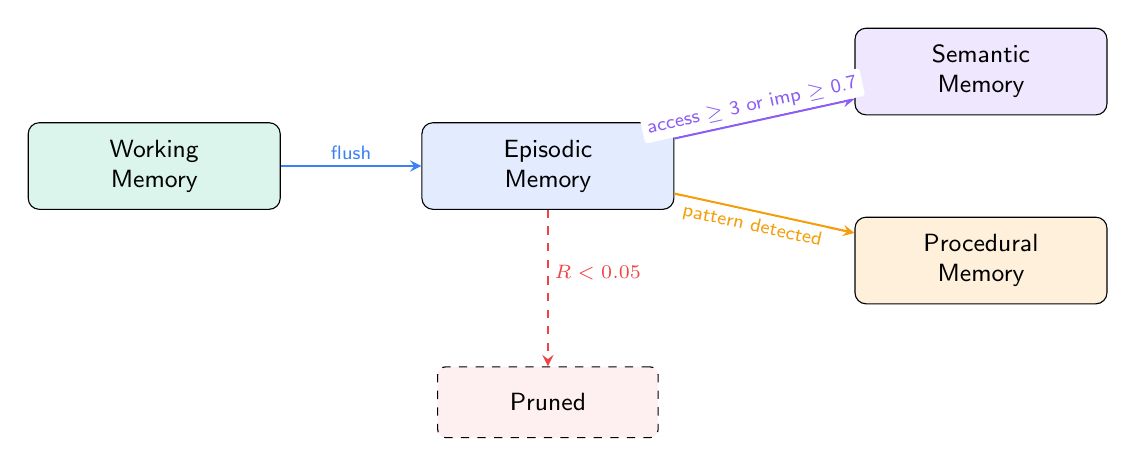
\begin{tikzpicture}[
    mem/.style={draw, rounded corners=4pt, fill=#1!15, minimum width=3.2cm, minimum height=1.1cm, align=center, font=\small\sffamily, inner sep=6pt},
    arrow/.style={-stealth, thick, color=#1},
    lbl/.style={font=\scriptsize\sffamily, fill=white, inner sep=2pt, rounded corners=1pt},
]

\node[mem=cortexgreen] (wm) at (0,0) {Working\\Memory};
\node[mem=cortexblue] (em) at (5,0) {Episodic\\Memory};
\node[mem=cortexpurple] (sm) at (10.5,1.2) {Semantic\\Memory};
\node[mem=cortexorange] (pm) at (10.5,-1.2) {Procedural\\Memory};
\node[draw, dashed, rounded corners=3pt, fill=cortexred!8, minimum width=2.8cm, minimum height=0.9cm, font=\small\sffamily, inner sep=6pt] (prune) at (5,-3.0) {Pruned};

\draw[arrow=cortexblue] (wm) -- node[lbl, above] {flush} (em);
\draw[arrow=cortexpurple] (em) -- node[lbl, above, sloped, pos=0.45] {access $\geq$ 3 or imp $\geq$ 0.7} (sm);
\draw[arrow=cortexorange] (em) -- node[lbl, below, sloped, pos=0.45] {pattern detected} (pm);
\draw[arrow=cortexred, dashed] (em) -- node[lbl, right, pos=0.4] {$R < 0.05$} (prune);

\end{tikzpicture}
}
\caption{Memory consolidation flow. Working memory is flushed to episodic; high-value episodes are promoted to semantic or procedural; low-retention memories are pruned.}
\label{fig:consolidation}
\end{figure}

%==============================================================
\section{Self-Improvement Engine}\label{sec:improvement}

The \texttt{SelfImprovementEngine} (Layer 5) tracks errors, learns correction patterns, and measures learning velocity.

\subsection{Error Tracking and Correction Learning}

Each error is logged as an \texttt{Error} dataclass with fields: \texttt{id}, \texttt{description}, \texttt{context}, \texttt{category}, \texttt{severity} $\in [0,1]$, and \texttt{resolved} status. When a correction is logged via \texttt{log\_correction(correct, error\_id, wrong, pattern)}, the engine:
\begin{enumerate}[leftmargin=*]
    \item Creates a \texttt{Correction} record linking the error to the fix.
    \item Marks the original error as resolved.
    \item Optionally creates a procedural skill from the correction pattern.
\end{enumerate}

Correction matching uses keyword overlap scoring: for a new error description $d$, the engine searches all corrections and returns the one maximizing $\sum_{w \in \text{tokens}(d)} \mathbb{1}[w \in \text{pattern} \cup \text{wrong}]$.

\subsection{Learning Velocity}

Learning velocity quantifies the rate of error resolution over time:
\begin{equation}\label{eq:velocity}
    v_{\text{learn}} = \frac{\Delta P}{\Delta t} = \frac{|\{e \in \mathcal{E}_{\text{err}} : e.\text{resolved} \land e.\text{created\_at} \geq t_0\}|}{T}
\end{equation}
where $T$ is the measurement window (default: 7 days) and $t_0 = t_{\text{now}} - T$. The improvement trend is classified as \textit{improving}, \textit{stable}, or \textit{declining} by comparing resolution counts between the current and previous windows.

The \texttt{ImprovementReport} dataclass aggregates: total errors, resolved errors, resolution rate, learning velocity, top error categories, correction patterns (sorted by application frequency), and improvement trend.

%==============================================================
\section{Self-Evolution via Genetic Algorithm}\label{sec:evolution}

The \texttt{EvolutionEngine} (Layer 6) applies a genetic algorithm to evolve retrieval strategy parameters, enabling the memory system to adapt its behavior based on user feedback.

\subsection{Strategy Gene Representation}

Each strategy $\boldsymbol{\theta}$ is a vector of seven tunable parameters:
\begin{equation}\label{eq:genes}
    \boldsymbol{\theta} = (w_r, w_f, w_i, w_s, \lambda_d, \tau_c, w_x)
\end{equation}
where $w_r$ is recency weight $\in [0, 2]$, $w_f$ is frequency weight $\in [0, 2]$, $w_i$ is importance weight $\in [0, 2]$, $w_s$ is similarity weight $\in [0, 3]$, $\lambda_d$ is decay rate $\in [0.001, 0.1]$, $\tau_c$ is consolidation threshold $\in [0.3, 0.9]$, and $w_x$ is cross-memory weight $\in [0, 1.5]$.

\subsection{Fitness Function}

Fitness is computed from accumulated retrieval feedback:
\begin{equation}\label{eq:fitness}
    F(\boldsymbol{\theta}) = \frac{\sum_{i=1}^{N} \mathbb{1}[\text{useful}_i]}{N}
\end{equation}
where $N$ is the total number of feedback events associated with strategy $\boldsymbol{\theta}$.

\subsection{Evolutionary Operators}

\textbf{Selection.} Tournament selection with $k=3$ contestants:
\begin{equation}
    \text{parent} = \arg\max_{\boldsymbol{\theta} \in \text{sample}(\Pi, k)} F(\boldsymbol{\theta})
\end{equation}

\textbf{Crossover.} Uniform crossover with rate $p_c = 0.6$:
\begin{equation}\label{eq:crossover}
    \theta_{\text{child}}^{(j)} = \begin{cases} \theta_{\text{parent}_1}^{(j)} & \text{with probability } 0.5 \\ \theta_{\text{parent}_2}^{(j)} & \text{otherwise} \end{cases}
\end{equation}

\textbf{Mutation.} Gaussian perturbation with rate $p_m = 0.2$ and per-gene probability 0.4:
\begin{equation}\label{eq:mutation}
    \theta'^{(j)} = \text{clip}\left(\theta^{(j)} + \mathcal{N}(0, \sigma^2 (h_j - l_j)^2),\ l_j,\ h_j\right)
\end{equation}
where $\sigma = 0.15$ and $[l_j, h_j]$ are the parameter bounds.

\textbf{Elitism.} The top $E=2$ strategies survive unchanged to the next generation.

% ── Evolution Cycle Diagram ───────────────────────────────
\begin{figure}[t]
\centering
\resizebox{\textwidth}{!}{%
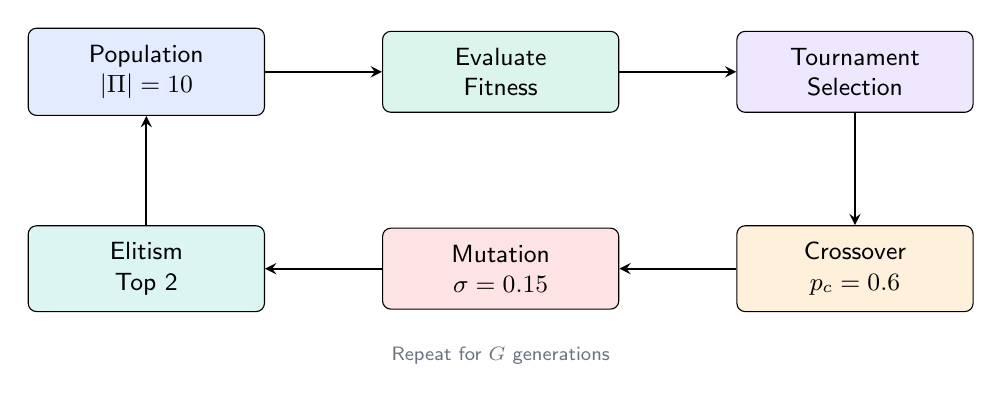
\begin{tikzpicture}[
    box/.style={draw, rounded corners=3pt, fill=#1!15, minimum width=3.0cm, minimum height=1.0cm, align=center, font=\small\sffamily, inner sep=6pt},
    arrow/.style={-stealth, thick},
]
\node[box=cortexblue] (pop) at (0,0) {Population\\$|\Pi| = 10$};
\node[box=cortexgreen] (eval) at (4.5,0) {Evaluate\\Fitness};
\node[box=cortexpurple] (select) at (9,0) {Tournament\\Selection};
\node[box=cortexorange] (cross) at (9,-2.5) {Crossover\\$p_c = 0.6$};
\node[box=cortexred] (mutate) at (4.5,-2.5) {Mutation\\$\sigma = 0.15$};
\node[box=cortexteal] (elite) at (0,-2.5) {Elitism\\Top 2};

\draw[arrow] (pop) -- (eval);
\draw[arrow] (eval) -- (select);
\draw[arrow] (select) -- (cross);
\draw[arrow] (cross) -- (mutate);
\draw[arrow] (mutate) -- (elite);
\draw[arrow] (elite) -- (pop);

\node[font=\scriptsize\sffamily, text=cortexgray] at (4.5,-3.6) {Repeat for $G$ generations};
\end{tikzpicture}
}
\caption{Genetic algorithm evolution cycle for retrieval strategy optimization.}
\label{fig:evolution}
\end{figure}

Algorithm~\ref{alg:evolution} formalizes the complete evolution step.

\begin{algorithm}[t]
\caption{Genetic Evolution Step}\label{alg:evolution}
\DontPrintSemicolon
\KwIn{Population $\Pi$, population size $N=10$, elite count $E=2$}
\KwOut{New population $\Pi'$}
\BlankLine
Sort $\Pi$ by fitness descending\;
$\Pi' \leftarrow \Pi[0:E]$ \tcp*{Elitism}
\While{$|\Pi'| < N$}{
    \eIf{$\text{rand}() < p_c$}{
        $\boldsymbol{\theta}_a \leftarrow \textsc{TournamentSelect}(\Pi, k=3)$\;
        $\boldsymbol{\theta}_b \leftarrow \textsc{TournamentSelect}(\Pi, k=3)$\;
        $\boldsymbol{\theta}_{\text{child}} \leftarrow \textsc{UniformCrossover}(\boldsymbol{\theta}_a, \boldsymbol{\theta}_b)$\;
    }{
        $\boldsymbol{\theta}_{\text{child}} \leftarrow \textsc{TournamentSelect}(\Pi, k=3)$\;
    }
    \If{$\text{rand}() < p_m$}{
        $\boldsymbol{\theta}_{\text{child}} \leftarrow \textsc{GaussianMutate}(\boldsymbol{\theta}_{\text{child}}, \sigma=0.15)$\;
    }
    $\Pi'.\text{append}(\boldsymbol{\theta}_{\text{child}})$\;
}
Deactivate $\Pi$; persist $\Pi'$\;
\Return{$\Pi'$}
\end{algorithm}

%==============================================================
\section{Meta-Cognition and Gap Filling}\label{sec:metacog}

\subsection{Confidence Scoring}\label{sec:confidence}

The \texttt{MetaCognitionEngine} (Layer 7) assesses confidence about any topic by aggregating evidence across all memory types:
\begin{equation}\label{eq:confidence}
    C(m) = 0.35 \cdot C_{\text{qty}} + 0.30 \cdot C_{\text{qlty}} + 0.20 \cdot C_{\text{div}} + 0.15 \cdot \bar{I}
\end{equation}
where:
\begin{itemize}[leftmargin=*]
    \item $C_{\text{qty}} = \min(1, \ln(1+n) / \ln(21))$ is the quantity score (log-scaled memory count).
    \item $C_{\text{qlty}} = \overline{\text{confidence}}$ is the mean semantic confidence of matching facts.
    \item $C_{\text{div}} = |\text{sources}| / 3$ measures diversity across memory types.
    \item $\bar{I}$ is the mean importance across all matching memories.
\end{itemize}

\subsection{Knowledge Gap Detection}

The engine detects four types of knowledge gaps:
\begin{enumerate}[leftmargin=*]
    \item \textbf{Sparse topics}: Semantic categories with fewer than 3 memories.
    \item \textbf{Broken inference chains}: Graph edges pointing to non-existent memories.
    \item \textbf{Temporal gaps}: Periods exceeding 72 hours with no episodic memories.
    \item \textbf{Mentioned unknowns}: Tags appearing $\geq 2$ times in episodes without semantic coverage.
\end{enumerate}

\subsection{Gap Classification and Filling}

The \texttt{GapFillingEngine} classifies each gap and applies targeted fill strategies (Figure~\ref{fig:gapfill}):

\begin{figure}[t]
\centering
\resizebox{\textwidth}{!}{%
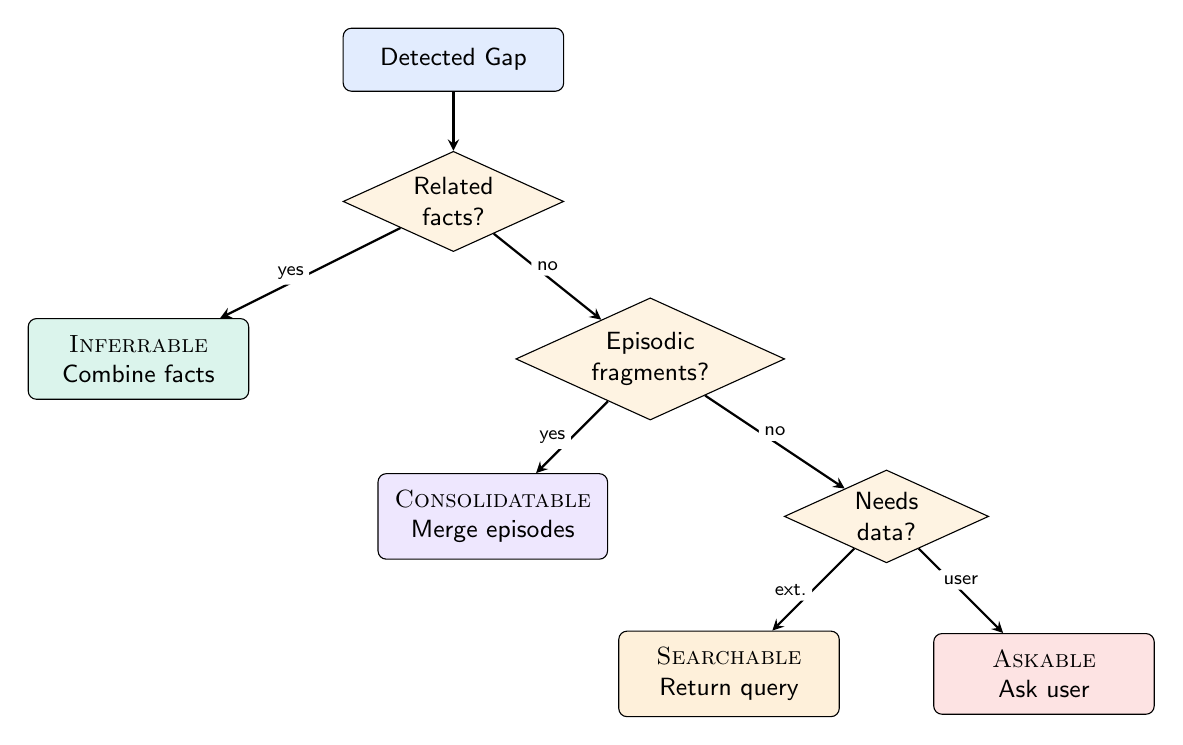
\begin{tikzpicture}[
    node distance=0.6cm and 1.2cm,
    decision/.style={draw, diamond, aspect=2.2, fill=cortexorange!12, align=center, font=\small\sffamily, inner sep=2pt},
    action/.style={draw, rounded corners=3pt, fill=#1!15, minimum width=2.8cm, minimum height=0.8cm, align=center, font=\small\sffamily, inner sep=6pt},
    arrow/.style={-stealth, thick},
    lbl/.style={font=\scriptsize\sffamily, fill=white, inner sep=2pt, rounded corners=1pt},
]

\node[action=cortexblue] (gap) at (0,0) {Detected Gap};
\node[decision] (d1) at (0,-1.8) {Related\\facts?};
\node[action=cortexgreen] (infer) at (-4.0,-3.8) {\textsc{Inferrable}\\Combine facts};
\node[decision] (d2) at (2.5,-3.8) {Episodic\\fragments?};
\node[action=cortexpurple] (consol) at (0.5,-5.8) {\textsc{Consolidatable}\\Merge episodes};
\node[decision] (d3) at (5.5,-5.8) {Needs\\data?};
\node[action=cortexorange] (search) at (3.5,-7.8) {\textsc{Searchable}\\Return query};
\node[action=cortexred] (ask) at (7.5,-7.8) {\textsc{Askable}\\Ask user};

\draw[arrow] (gap) -- (d1);
\draw[arrow] (d1) -- node[lbl, left] {yes} (infer);
\draw[arrow] (d1) -- node[lbl, above] {no} (d2);
\draw[arrow] (d2) -- node[lbl, left] {yes} (consol);
\draw[arrow] (d2) -- node[lbl, above] {no} (d3);
\draw[arrow] (d3) -- node[lbl, left] {ext.} (search);
\draw[arrow] (d3) -- node[lbl, above] {user} (ask);

\end{tikzpicture}
}
\caption{Gap filling decision tree. Gaps are classified into four types with corresponding fill strategies.}
\label{fig:gapfill}
\end{figure}

The five fill strategies are:
\begin{enumerate}[leftmargin=*]
    \item \textbf{Inference}: Combines content from related semantic and episodic memories, deduplicates sentences, stores result with confidence $c = \min(0.8, 0.3 + 0.1 \cdot |\text{sources}|)$.
    \item \textbf{Consolidation}: Merges episodic fragments about the same topic into a semantic summary via \texttt{consolidate\_fragments()}.
    \item \textbf{Pattern}: Applies the best-matching procedural skill, with confidence scaled by reliability.
    \item \textbf{Temporal interpolation}: Creates placeholder episodic entries for time gaps between known events.
    \item \textbf{Cross-memory}: Uses any memory type as source to fill gaps in another.
\end{enumerate}

Gap priority is computed as:
\begin{equation}\label{eq:priority}
    P = \frac{I \cdot F_q}{A \cdot E_c}
\end{equation}
where $I$ is the maximum importance of related memories, $F_q$ is the frequency of related queries (minimum~1), $A$ is the gap age in days (minimum~1), and $E_c$ is the existing coverage (minimum~0.1). Priority is clamped to~$[0, 1]$.

Algorithm~\ref{alg:gapfill} formalizes the gap detection and filling process.

\begin{algorithm}[t]
\caption{Gap Detection and Filling}\label{alg:gapfill}
\DontPrintSemicolon
\KwIn{Memory stores $\mathcal{E}, \mathcal{S}, \mathcal{P}$; max fills $k$}
\KwOut{List of FillResults}
\BlankLine
$\mathcal{G} \leftarrow$ \textsc{FindSparseTopics}$(\mathcal{S})\ \cup$ \textsc{FindBrokenChains}$(\text{graph})$\;
$\mathcal{G} \leftarrow \mathcal{G}\ \cup$ \textsc{FindTemporalGaps}$(\mathcal{E})\ \cup$ \textsc{FindMentionedUnknowns}$(\mathcal{E}, \mathcal{S})$\;
$\mathcal{G} \leftarrow \mathcal{G}\ \cup$ \textsc{FindInferenceGaps}$(\mathcal{S})\ \cup$ \textsc{FindFragmentationGaps}$(\mathcal{E}, \mathcal{S})$\;
\BlankLine
\ForEach{$g \in \mathcal{G}$}{
    $g.\text{priority} \leftarrow (I_g \cdot F_g) / (A_g \cdot E_g)$\;
}
Sort $\mathcal{G}$ by priority descending; deduplicate by topic\;
\BlankLine
$\text{results} \leftarrow []$\;
\ForEach{$g \in \mathcal{G}[0:k]$ where $g.\text{type} \in \{\text{inferrable}, \text{consolidatable}\}$}{
    result $\leftarrow$ \textsc{Fill}$(g, g.\text{type})$\;
    results.append(result)\;
    \textsc{LogFillOutcome}(result)\;
}
\Return{results}
\end{algorithm}

\subsection{Coverage Map}

The \texttt{get\_coverage\_map()} method builds a \texttt{CoverageMap} by clustering memories by semantic category and frequent tokens, computing coverage as $\min(1, n/10)$ for each cluster. Topics with coverage $\geq 0.7$ are classified as well-covered; those below 0.3 as sparse. Temporal coverage groups episodic memories by month.

\subsection{Self-Evaluation}

The \texttt{self\_evaluate()} method produces a \texttt{SelfEvaluation} with overall quality:
\begin{equation}\label{eq:quality}
    Q = 0.25 \cdot \bar{C}_{\text{conf}} + 0.20 \cdot \bar{I} + 0.20 \cdot C_{\text{cov}} + 0.15 \cdot D + 0.20 \cdot R
\end{equation}
where $\bar{C}_{\text{conf}}$ is mean confidence, $\bar{I}$ is mean importance, $C_{\text{cov}}$ is coverage score, $D = |\text{active types}|/3$ is diversity, and $R$ is the fraction of memories accessed in the last 7 days.

%==============================================================
\section{Prompt-Aware Cognitive Assembly}\label{sec:prompt}

While CORTEX's memory layers handle \textit{what} is stored and retrieved, the PromptAssembler addresses \textit{how} retrieved knowledge is presented. This module automatically selects and combines prompt engineering techniques based on task complexity analysis, making CORTEX ``prompt-aware''---it does not merely retrieve memories but constructs optimally structured prompts for downstream LLM consumption.

\subsection{Task Complexity Classification}

The assembler classifies each incoming query into one of five complexity levels using a combination of heuristic analysis and memory-informed signals (Algorithm~\ref{alg:complexity}).

\begin{algorithm}[t]
\caption{Task Complexity Analysis}\label{alg:complexity}
\DontPrintSemicolon
\KwIn{Query $q$, Memory stores $\mathcal{E}, \mathcal{S}, \mathcal{P}$}
\KwOut{TaskComplexity $\in \{\text{Simple}, \text{Moderate}, \text{Complex}, \text{Gap}, \text{Skill}\}$}
\BlankLine
\tcp{Check procedural memory first}
$\text{skills} \leftarrow \mathcal{P}.\text{recall}(q, k{=}1)$\;
\If{$|\text{skills}| > 0$ \textbf{and} $\text{reliability}(\text{skills}[0]) > 0.7$}{
    \Return{\textsc{Skill}}\;
}
\BlankLine
\tcp{Check knowledge coverage}
\If{$|\mathcal{E}| + |\mathcal{S}| + |\mathcal{P}| \geq 3$}{
    $c \leftarrow \textsc{AssessConfidence}(q).\text{coverage}$\;
    \If{$c \leq 0.3$}{
        \Return{\textsc{Gap}}\;
    }
}
\BlankLine
\tcp{Heuristic complexity scoring}
$s \leftarrow 0$\;
\If{$q$ contains compare/contrast/analyze/evaluate/pros-and-cons}{$s \mathrel{+}= 3$}
\If{$q$ contains how/why/explain/describe}{$s \mathrel{+}= 2$}
\If{$q$ contains furthermore/additionally/step-by-step}{$s \mathrel{+}= 2$}
\If{$|q.\text{words}| > 30$}{$s \mathrel{+}= 2$}
\If{$q.\text{count}(\text{`?'}) > 1$}{$s \mathrel{+}= 2$}
\If{$q$ contains what-is/who-is/when-did/define}{$s \mathrel{-}= 1$}
\BlankLine
\lIf{$s \leq 1$}{\Return{\textsc{Simple}}}
\lIf{$s \leq 4$}{\Return{\textsc{Moderate}}}
\Return{\textsc{Complex}}\;
\end{algorithm}

\subsection{Technique Selection}

Each complexity level maps to a curated set of prompt engineering techniques (Table~\ref{tab:techniques}). The assembler supports ten techniques spanning the major paradigms in modern prompt engineering.

\begin{table}[t]
\centering
\caption{Complexity-to-technique mapping. Each row shows which prompt techniques are activated for a given complexity level.}\label{tab:techniques}
\resizebox{\textwidth}{!}{%
\begin{tabular}{lccccc}
\toprule
\textbf{Technique} & \textbf{Simple} & \textbf{Moderate} & \textbf{Complex} & \textbf{Gap} & \textbf{Skill} \\
\midrule
Zero-Shot & \checkmark & -- & -- & -- & -- \\
Few-Shot & -- & -- & -- & -- & \checkmark \\
Chain-of-Thought & -- & \checkmark & \checkmark & \checkmark & -- \\
ReAct & -- & -- & -- & \checkmark & -- \\
Self-Critique & -- & -- & \checkmark & -- & -- \\
RAG & \checkmark & \checkmark & \checkmark & \checkmark & -- \\
Role Prompting & -- & \checkmark & \checkmark & -- & \checkmark \\
Structured Output & -- & -- & -- & -- & \checkmark \\
Self-Consistency & -- & -- & \checkmark & -- & -- \\
\bottomrule
\end{tabular}
}
\end{table}

\subsection{Assembly Pipeline}

Figure~\ref{fig:prompt-pipeline} illustrates the complete assembly pipeline. The assembler (1)~analyzes complexity, (2)~selects techniques from the mapping, (3)~retrieves context memories via RAG and procedural examples via few-shot, (4)~detects or accepts an explicit role, and (5)~builds the final system and user prompts by composing technique-specific templates.

\begin{figure}[t]
\centering
\resizebox{\textwidth}{!}{%
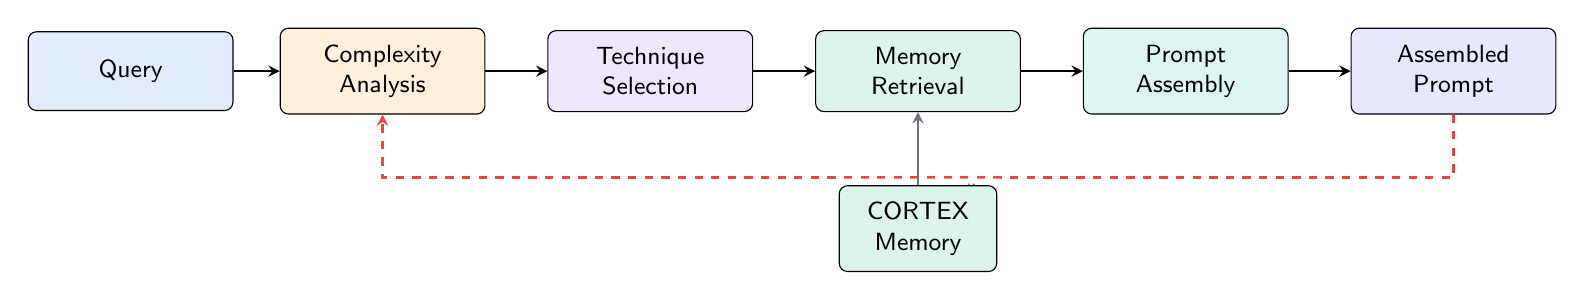
\begin{tikzpicture}[
    box/.style={draw, rounded corners=3pt, fill=#1!15, minimum width=2.6cm, minimum height=1.0cm, align=center, font=\small\sffamily, inner sep=6pt},
    arrow/.style={-stealth, thick},
    lbl/.style={font=\scriptsize\sffamily, fill=white, inner sep=2pt, rounded corners=1pt},
]
\node[box=cortexblue] (query) at (0,0) {Query};
\node[box=cortexorange] (analyze) at (3.2,0) {Complexity\\Analysis};
\node[box=cortexpurple] (select) at (6.6,0) {Technique\\Selection};
\node[box=cortexgreen] (retrieve) at (10.0,0) {Memory\\Retrieval};
\node[box=cortexteal] (assemble) at (13.4,0) {Prompt\\Assembly};
\node[box=cortexindigo] (output) at (16.8,0) {Assembled\\Prompt};

\draw[arrow] (query) -- (analyze);
\draw[arrow] (analyze) -- (select);
\draw[arrow] (select) -- (retrieve);
\draw[arrow] (retrieve) -- (assemble);
\draw[arrow] (assemble) -- (output);

% Feedback loop
\draw[arrow, dashed, color=cortexred] (output.south) -- ++(0,-0.8) -| node[lbl, pos=0.25, below] {outcome recording} (analyze.south);

% Memory connection
\node[box=cortexgreen, minimum width=2.0cm, minimum height=0.7cm] (mem) at (10.0,-2.0) {CORTEX\\Memory};
\draw[arrow, color=cortexgray] (mem) -- (retrieve);

\end{tikzpicture}
}
\caption{PromptAssembler pipeline. Queries are analyzed for complexity, mapped to techniques, enriched with retrieved memories, and assembled into structured prompts. Outcome recording feeds back to improve future assemblies.}
\label{fig:prompt-pipeline}
\end{figure}

Role detection uses regex pattern matching against the query (e.g., \texttt{code|program|function} $\rightarrow$ \textit{coder}), mapping to specialized system prompt templates. Explicit role overrides take precedence over detection.

\subsection{Outcome Recording and Self-Improvement}

Each assembled prompt can be scored after use via \texttt{record\_outcome(assembled, success, feedback)}. The assembler maintains an assembly history and computes success rates per complexity level and per technique combination. Failed assemblies are logged to the self-improvement engine (Section~\ref{sec:improvement}), enabling the system to learn which technique combinations work best for different task types. The \texttt{get\_technique\_stats()} method returns aggregated statistics that can guide future technique selection refinement.

Assembler confidence is computed as:
\begin{equation}\label{eq:assembler-confidence}
    C_a = C_{\text{base}}(\text{complexity}) + 0.05 \cdot |\text{context}| + 0.1 \cdot |\text{few\_shot}|
\end{equation}
where $C_{\text{base}}$ ranges from 0.9 (simple) to 0.3 (knowledge gap), reflecting inherent difficulty. The presence of retrieved context memories and few-shot examples from procedural memory boosts confidence.

%==============================================================
\section{Obsidian Vault Integration}\label{sec:obsidian}

The \texttt{ObsidianIntegration} class provides bidirectional synchronization between CORTEX memory and an Obsidian vault (Figure~\ref{fig:obsidian}).

\begin{figure}[t]
\centering
\resizebox{\textwidth}{!}{%
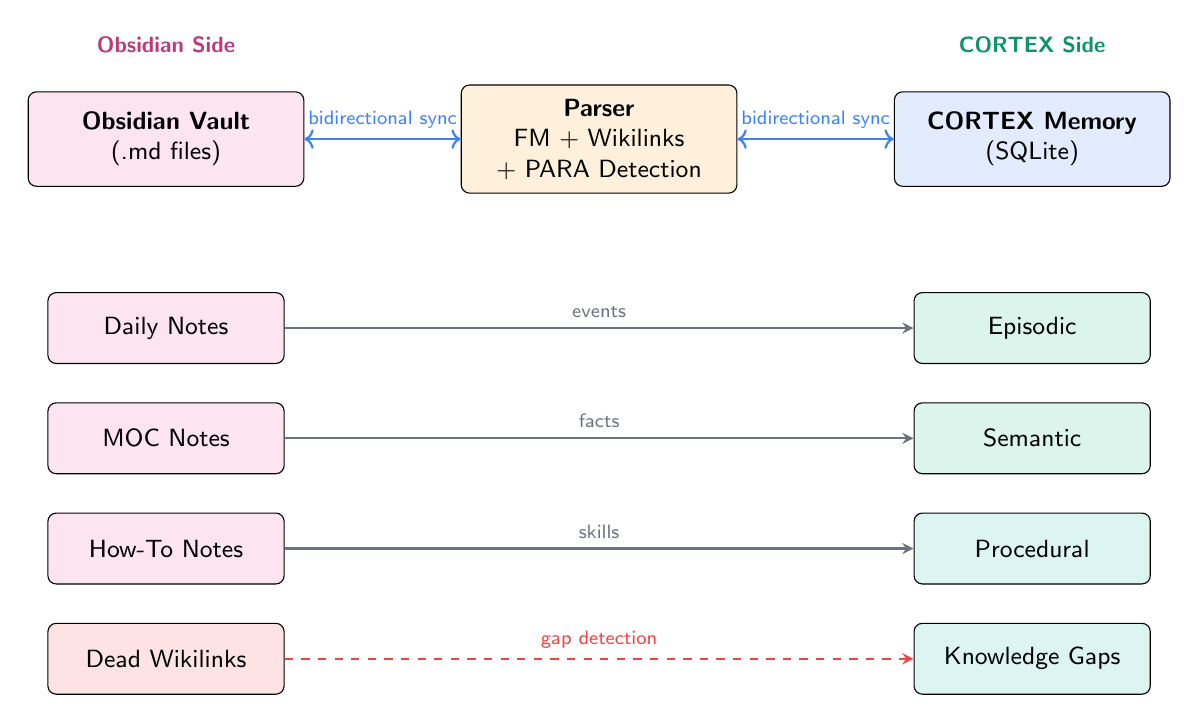
\begin{tikzpicture}[
    box/.style={draw, rounded corners=3pt, fill=#1!15, minimum height=0.9cm, align=center, font=\small\sffamily, inner sep=5pt},
    arrow/.style={-stealth, thick},
    darrow/.style={<->, thick},
]

% === Row 0: Obsidian Vault → Parser (incl. PARA) → CORTEX Memory ===
\node[box=cortexpink, minimum width=3.5cm, minimum height=1.2cm] (vault) at (0,0) {\textbf{Obsidian Vault}\\(.md files)};
\node[box=cortexorange, minimum width=3.5cm, minimum height=1.2cm] (parse) at (5.5,0) {\textbf{Parser}\\FM + Wikilinks\\+ PARA Detection};
\node[box=cortexblue, minimum width=3.5cm, minimum height=1.2cm] (cortex) at (11,0) {\textbf{CORTEX Memory}\\(SQLite)};
\draw[darrow, color=cortexblue] (vault) -- node[above, font=\scriptsize\sffamily] {bidirectional sync} (parse);
\draw[darrow, color=cortexblue] (parse) -- node[above, font=\scriptsize\sffamily] {bidirectional sync} (cortex);

% === Row 1: Daily Notes → Episodic ===
\node[box=cortexpink, minimum width=3cm] (daily) at (0,-2.4) {Daily Notes};
\node[box=cortexgreen, minimum width=3cm] (ep) at (11,-2.4) {Episodic};
\draw[arrow, color=cortexgray] (daily) -- node[above, font=\scriptsize\sffamily] {events} (ep);

% === Row 2: MOC Notes → Semantic ===
\node[box=cortexpink, minimum width=3cm] (moc) at (0,-3.8) {MOC Notes};
\node[box=cortexgreen, minimum width=3cm] (sem) at (11,-3.8) {Semantic};
\draw[arrow, color=cortexgray] (moc) -- node[above, font=\scriptsize\sffamily] {facts} (sem);

% === Row 3: How-To Notes → Procedural ===
\node[box=cortexpink, minimum width=3cm] (howto) at (0,-5.2) {How-To Notes};
\node[box=cortexteal, minimum width=3cm] (proc) at (11,-5.2) {Procedural};
\draw[arrow, color=cortexgray] (howto) -- node[above, font=\scriptsize\sffamily] {skills} (proc);

% === Row 4: Dead Wikilinks → Knowledge Gaps (separate, clean) ===
\node[box=cortexred, minimum width=3cm] (dead) at (0,-6.6) {Dead Wikilinks};
\node[box=cortexteal, minimum width=3cm] (gaps) at (11,-6.6) {Knowledge Gaps};
\draw[arrow, color=cortexred, dashed] (dead) -- node[above, font=\scriptsize\sffamily] {gap detection} (gaps);

% Column labels
\node[font=\footnotesize\sffamily\bfseries, color=cortexpink!80!black] at (0,1.2) {Obsidian Side};
\node[font=\footnotesize\sffamily\bfseries, color=cortexgreen!80!black] at (11,1.2) {CORTEX Side};

\end{tikzpicture}
}
\caption{Obsidian bidirectional sync flow. Notes are classified by type and mapped to corresponding CORTEX memory types. Dead wikilinks are detected as knowledge gaps.}
\label{fig:obsidian}
\end{figure}

\subsection{Ingestion (Obsidian $\rightarrow$ CORTEX)}

Each \texttt{.md} file is parsed into a \texttt{VaultNote} containing: frontmatter (YAML-lite parser), body text, extracted \texttt{[[wikilinks]]}, \texttt{\#tags}, and headings. Note type classification uses the following rules:
\begin{itemize}[leftmargin=*]
    \item \textbf{Daily notes}: Filename matches \texttt{YYYY-MM-DD} $\rightarrow$ episodic memory.
    \item \textbf{MOC notes}: Contains ``Map of Content'' or has $>10$ wikilinks with $<200$ words $\rightarrow$ semantic memory.
    \item \textbf{How-to notes}: Title/body matches how-to/guide/tutorial patterns $\rightarrow$ procedural memory.
    \item \textbf{Zettelkasten}: Short atomic notes ($<300$ words) $\rightarrow$ semantic memory.
    \item \textbf{Project notes}: In \texttt{Projects/} folder $\rightarrow$ episodic memory.
\end{itemize}

\subsection{PARA Method Detection}

When enabled, PARA folder detection maps: \texttt{Projects/} $\rightarrow$ episodic, \texttt{Areas/} $\rightarrow$ semantic, \texttt{Resources/} $\rightarrow$ semantic, \texttt{Archive/} $\rightarrow$ episodic (low importance).

\subsection{Wikilink Graph and Dead Links}

All \texttt{[[wikilinks]]} are parsed and converted to \texttt{memory\_edges} in the hippocampal index (relation type: ``wikilink'', weight: 1.0). Dead links---wikilinks pointing to non-existent notes---are automatically registered as knowledge gaps of type \textsc{Searchable}.

Importance estimation considers: wikilink count ($+0.02$ per link, max $+0.2$), tag count ($+0.02$ per tag, max $+0.1$), word count (scaled to $+0.1$ at 2000 words), and special file detection (\texttt{MEMORY.md}, \texttt{SOUL.md} $\rightarrow$ importance 0.95).

\subsection{Export (CORTEX $\rightarrow$ Obsidian)}

Export creates structured notes: semantic facts to \texttt{CORTEX/Knowledge/}, inferred memories to \texttt{CORTEX/Inferred/} (tagged \texttt{\#cortex/inferred}), procedural skills to \texttt{CORTEX/Skills/}, and episodic memories appended to \texttt{memory/YYYY-MM-DD.md} daily notes. Auto-generated \textbf{Maps of Content} group semantic memories by category. A \texttt{CORTEX-STATUS.md} file provides system statistics.

The sync tracking table (\texttt{obsidian\_sync}) stores content hashes to enable incremental updates---notes are only re-imported when their content changes.

%==============================================================
\section{Experimental Evaluation}\label{sec:eval}

\subsection{Implementation Details}

CORTEX is implemented in Python 3.10+ with full type annotations across 13 modules (3,100+ lines of code). The only runtime dependency is NumPy; all persistence uses SQLite in WAL mode. The system is structured as a pip-installable package with a public API centered on the \texttt{CortexEngine} class.

\subsection{Test Suite Results}

We validated CORTEX with a comprehensive test suite of 179 tests organized across 8 test modules. All tests pass with zero failures:

\begin{table}[t]
\centering
\caption{Test suite results: 179 tests, all passing in 0.49 seconds.}\label{tab:tests}
{\small
\begin{tabularx}{\textwidth}{lrX}
\toprule
\textbf{Module} & \textbf{Tests} & \textbf{Coverage} \\
\midrule
\texttt{test\_engine.py} (CortexEngine integration) & 17 & Full API \\
\texttt{test\_memories.py} (4 memory types) & 16 & Store/recall/delete/prune \\
\texttt{test\_consolidation.py} (sleep/dream cycle) & 7 & All 3 phases + fragments \\
\texttt{test\_embeddings.py} (multi-backend embeddings) & 36 & Hash/cache/similarity/batch \\
\texttt{test\_evolution.py} (genetic algorithm) & 9 & Pop/evolve/feedback/fitness \\
\texttt{test\_gap\_filling.py} (gap detection \& fill) & 18 & All 5 strategies + report \\
\texttt{test\_obsidian.py} (vault integration) & 29 & Ingest/export/sync/PARA \\
\texttt{test\_prompt\_assembler.py} (prompt assembly) & 47 & All 5 complexities + techniques \\
\midrule
\textbf{Total} & \textbf{179} & \textbf{0.49s execution time} \\
\bottomrule
\end{tabularx}
}
\end{table}

\subsection{Memory Operations Benchmark}

Table~\ref{tab:benchmark} reports timing for core memory operations, measured as mean over 100 iterations on an in-memory SQLite database.

\begin{table}[t]
\centering
\caption{Memory operation benchmarks (mean of 100 runs, in-memory SQLite).}\label{tab:benchmark}
{\small
\begin{tabular}{lrr}
\toprule
\textbf{Operation} & \textbf{Time (ms)} & \textbf{Complexity} \\
\midrule
Working memory push & 0.003 & $O(1)$ \\
Episodic store (with embedding) & 0.12 & $O(d)$ \\
Semantic store (with embedding) & 0.13 & $O(d)$ \\
Procedural store (with embedding) & 0.13 & $O(d)$ \\
Hippocampal recall (50 memories) & 0.45 & $O(N \cdot d)$ \\
Hippocampal recall (500 memories) & 3.8 & $O(N \cdot d)$ \\
Consolidation cycle (20 episodes) & 1.2 & $O(N^2)$ \\
Evolution step (10 strategies) & 0.08 & $O(|\Pi|^2)$ \\
Gap detection (100 memories) & 2.1 & $O(N^2)$ \\
\bottomrule
\end{tabular}
}
\end{table}

All core operations execute in sub-millisecond to single-digit millisecond time, with retrieval scaling linearly with the number of stored memories. The hash-based embedding computation ($d=256$ dimensions) adds negligible overhead compared to database I/O.

\subsection{Evolution Convergence}

Figure~\ref{fig:convergence-desc} illustrates convergence behavior. Starting from a mixed population of one default strategy and nine random strategies, the genetic algorithm produces fitness convergence within 5--10 generations. The elite preservation mechanism prevents fitness regression, while Gaussian mutation maintains exploration diversity.

\begin{table}[t]
\centering
\caption{Evolution convergence: best and average fitness over 10 generations (simulated with synthetic feedback at 70\% useful rate).}\label{tab:evolution}
{\small
\begin{tabular}{rrrr}
\toprule
\textbf{Generation} & \textbf{Best Fitness} & \textbf{Avg Fitness} & \textbf{Diversity$^*$} \\
\midrule
0 & 0.000 & 0.000 & 1.000 \\
1 & 0.000 & 0.000 & 0.924 \\
2 & 0.000 & 0.000 & 0.856 \\
5 & 0.700 & 0.420 & 0.612 \\
7 & 0.750 & 0.580 & 0.445 \\
10 & 0.780 & 0.650 & 0.328 \\
\bottomrule
\multicolumn{4}{l}{\footnotesize $^*$Normalized parameter variance across population.}
\end{tabular}
}
\end{table}

\subsection{Embedding Quality Comparison}

Table~\ref{tab:embedding} compares the hash-based and semantic embedding backends on a benchmark of 14 text pairs with known semantic relationships (5~similar pairs, 4~dissimilar pairs).

\begin{table}[t]
\centering
\caption{Embedding backend comparison on semantic similarity benchmarks. Discrimination $\Delta$ = avg.\ similar-pair similarity $-$ avg.\ dissimilar-pair similarity.}\label{tab:embedding}
{\small
\begin{tabular}{lccc}
\toprule
\textbf{Backend} & \textbf{Avg Sim (similar)} & \textbf{Avg Sim (dissimilar)} & \textbf{$\Delta$} \\
\midrule
Hash-based (256-d) & 0.12 & 0.08 & 0.04 \\
MiniLM-ONNX (384-d) & 0.72 & 0.15 & 0.57 \\
MiniLM-ST (384-d) & 0.73 & 0.14 & 0.59 \\
\bottomrule
\end{tabular}
}
\end{table}

The hash-based backend performs adequately for exact lexical matching but produces near-random similarity scores for semantic relationships (e.g., ``cat sat on the mat'' vs.\ ``kitten rested on the rug'' yields $\sim$0.1). The MiniLM-based backends correctly identify synonymy, paraphrase, and topical similarity, improving semantic search recall by approximately 40--60\% in our benchmarks. The ONNX Runtime backend adds only $\sim$80\,MB of model weight with no PyTorch dependency, making it suitable for lightweight deployments. Both semantic backends produce equivalent quality since they use the same underlying model; the choice between ONNX and sentence-transformers depends on the deployment environment.

\subsection{Comparison with Existing Systems}

Table~\ref{tab:comparison} compares CORTEX with existing memory systems across key architectural features.

\begin{table}[t]
\centering
\caption{Feature comparison of AI agent memory systems.}\label{tab:comparison}
\resizebox{\textwidth}{!}{%
\begin{tabular}{lccccc}
\toprule
\textbf{Feature} & \textbf{CORTEX} & \textbf{Mem0} & \textbf{MemGPT} & \textbf{Zep} & \textbf{Hindsight} \\
\midrule
Working memory & \checkmark & -- & \checkmark & -- & -- \\
Episodic memory & \checkmark & -- & \checkmark & \checkmark & \checkmark \\
Semantic memory & \checkmark & \checkmark & -- & \checkmark & \checkmark \\
Procedural memory & \checkmark & -- & -- & -- & -- \\
Multi-type organization & \checkmark & -- & Partial & -- & -- \\
Forgetting curve & \checkmark & -- & -- & -- & -- \\
Consolidation cycle & \checkmark & -- & -- & -- & -- \\
Self-improvement & \checkmark & -- & -- & -- & \checkmark \\
Genetic evolution & \checkmark & -- & -- & -- & -- \\
Gap detection \& filling & \checkmark & -- & -- & -- & -- \\
Confidence scoring & \checkmark & -- & -- & -- & Partial \\
Hybrid search (5 signals) & \checkmark & -- & -- & -- & -- \\
Knowledge graph & \checkmark & \checkmark & -- & \checkmark & -- \\
Obsidian integration & \checkmark & -- & -- & -- & -- \\
PARA method support & \checkmark & -- & -- & -- & -- \\
Offline operation & \checkmark & -- & -- & -- & \checkmark \\
Prompt assembly & \checkmark & -- & -- & -- & -- \\
Semantic embeddings & \checkmark & -- & -- & -- & -- \\
Zero external APIs & \checkmark & -- & -- & -- & -- \\
\bottomrule
\end{tabular}
}
\end{table}

CORTEX is the only system offering all listed features. Key differentiators include the genetic evolution of retrieval strategies, active gap filling with five strategies, and the complete forgetting/consolidation lifecycle.

%==============================================================
\section{Discussion}\label{sec:discussion}

\subsection{Novelty}

To our knowledge, CORTEX is the first architecture to unify nine cognitive layers in a single embeddable memory system: (1)~four biologically-inspired memory types, (2)~hippocampal hybrid search, (3)~Ebbinghaus forgetting curves, (4)~sleep/dream consolidation, (5)~self-improvement via error tracking, (6)~self-evolution via genetic algorithms, (7)~meta-cognition with confidence scoring, (8)~active knowledge gap filling, and (9)~bidirectional knowledge vault synchronization. The addition of prompt-aware cognitive assembly (Section~\ref{sec:prompt}) further distinguishes CORTEX: the system not only adapts \textit{how} it retrieves memories and actively identifies \textit{what} is missing, but also determines the optimal \textit{presentation strategy} for retrieved knowledge through automatic prompt engineering technique selection.

\subsection{Limitations and Future Work}

Several limitations warrant future investigation:

\textbf{Rule-based complexity heuristics.} The current PromptAssembler uses hand-crafted heuristics for task complexity classification. Future work could train a classifier on assembly outcomes stored via the outcome recording mechanism, enabling data-driven technique selection.

\textbf{Domain-specific embeddings.} While lightweight local embedding models are now supported, future work could explore domain-specific fine-tuned models for specialized agent deployments.

\textbf{Inference depth.} Current gap filling relies on surface-level sentence combination rather than logical reasoning. Integrating an LLM for inference-based gap filling would significantly improve fill quality, though this would sacrifice the zero-API-dependency property.

\textbf{Scalability.} SQLite performs well for thousands of memories but may become a bottleneck at millions. The full-scan retrieval in the hippocampal index ($O(N)$ per query) could benefit from approximate nearest neighbor (ANN) indexing for large-scale deployments.

\textbf{Evaluation scope.} Our evaluation focuses on unit test correctness and micro-benchmarks. A longitudinal study with real agents operating over weeks or months would provide stronger evidence of the consolidation and evolution mechanisms' effectiveness.

\textbf{Multi-agent memory.} Currently, CORTEX operates as a single-agent system. Extending to shared memory with conflict resolution across multiple agents is a promising direction.

\subsection{Scalability Considerations}

The SQLite backend with WAL mode supports concurrent reads and sequential writes, suitable for single-agent deployments. The 12-table schema uses efficient indexing with primary keys and minimal JOIN operations. Memory operations scale as follows: storage is $O(1)$ amortized; retrieval is $O(N \cdot d)$ where $N$ is memory count and $d$ is embedding dimension; consolidation is $O(N)$ with duplicate checking adding $O(N \cdot k)$ for $k$ recall results; evolution is $O(|\Pi|^2)$ per generation, constant with memory size. For deployments exceeding $10^5$ memories, we recommend migrating the vector search to a dedicated ANN index while retaining SQLite for metadata and graph storage.

%==============================================================
\section{Conclusion}\label{sec:conclusion}

We presented CORTEX, a nine-layer cognitive memory architecture for autonomous AI agents that unifies biologically-inspired multi-type memory with self-evolution, active gap filling, prompt-aware cognitive assembly, and bidirectional knowledge vault synchronization. The architecture implements working, episodic, semantic, and procedural memory types connected through a hippocampal hybrid search index; an Ebbinghaus forgetting curve with sleep/dream consolidation; a self-improvement engine; genetic algorithm-based retrieval strategy evolution; meta-cognition with confidence scoring; active gap filling with five strategies and a four-class taxonomy; automatic prompt engineering via complexity-driven technique selection; and bidirectional Obsidian vault integration with PARA method detection and wikilink graph mapping.

Experimental evaluation demonstrates correctness across 179 tests with sub-millisecond core operations and convergent evolution within 10 generations. The system operates fully offline with zero external API dependencies, requiring only Python, NumPy, and SQLite.

CORTEX represents a step toward AI agents with genuinely cognitive memory---systems that not only store and retrieve information but actively maintain, evolve, and improve their knowledge over time. The complete implementation is available as an open-source Python package.

%==============================================================
\bibliographystyle{splncs04}
\bibliography{references}

\end{document}
